\documentclass{article}

\usepackage{graphicx}
\usepackage{tikz}
\usepackage{tikzsymbols}
\usetikzlibrary{calc,patterns,shapes.geometric}
\pagestyle{empty}
\usepackage[margin=0pt]{geometry}
\geometry{papersize={14in,12in}}

\def\centerarc[#1](#2)(#3:#4:#5){\draw[#1] ($(#2)+({#5*cos(#3)},{#5*sin(#3)})$) arc (#3:#4:#5);}

\begin{document}
	\begin{figure}
		\centering
		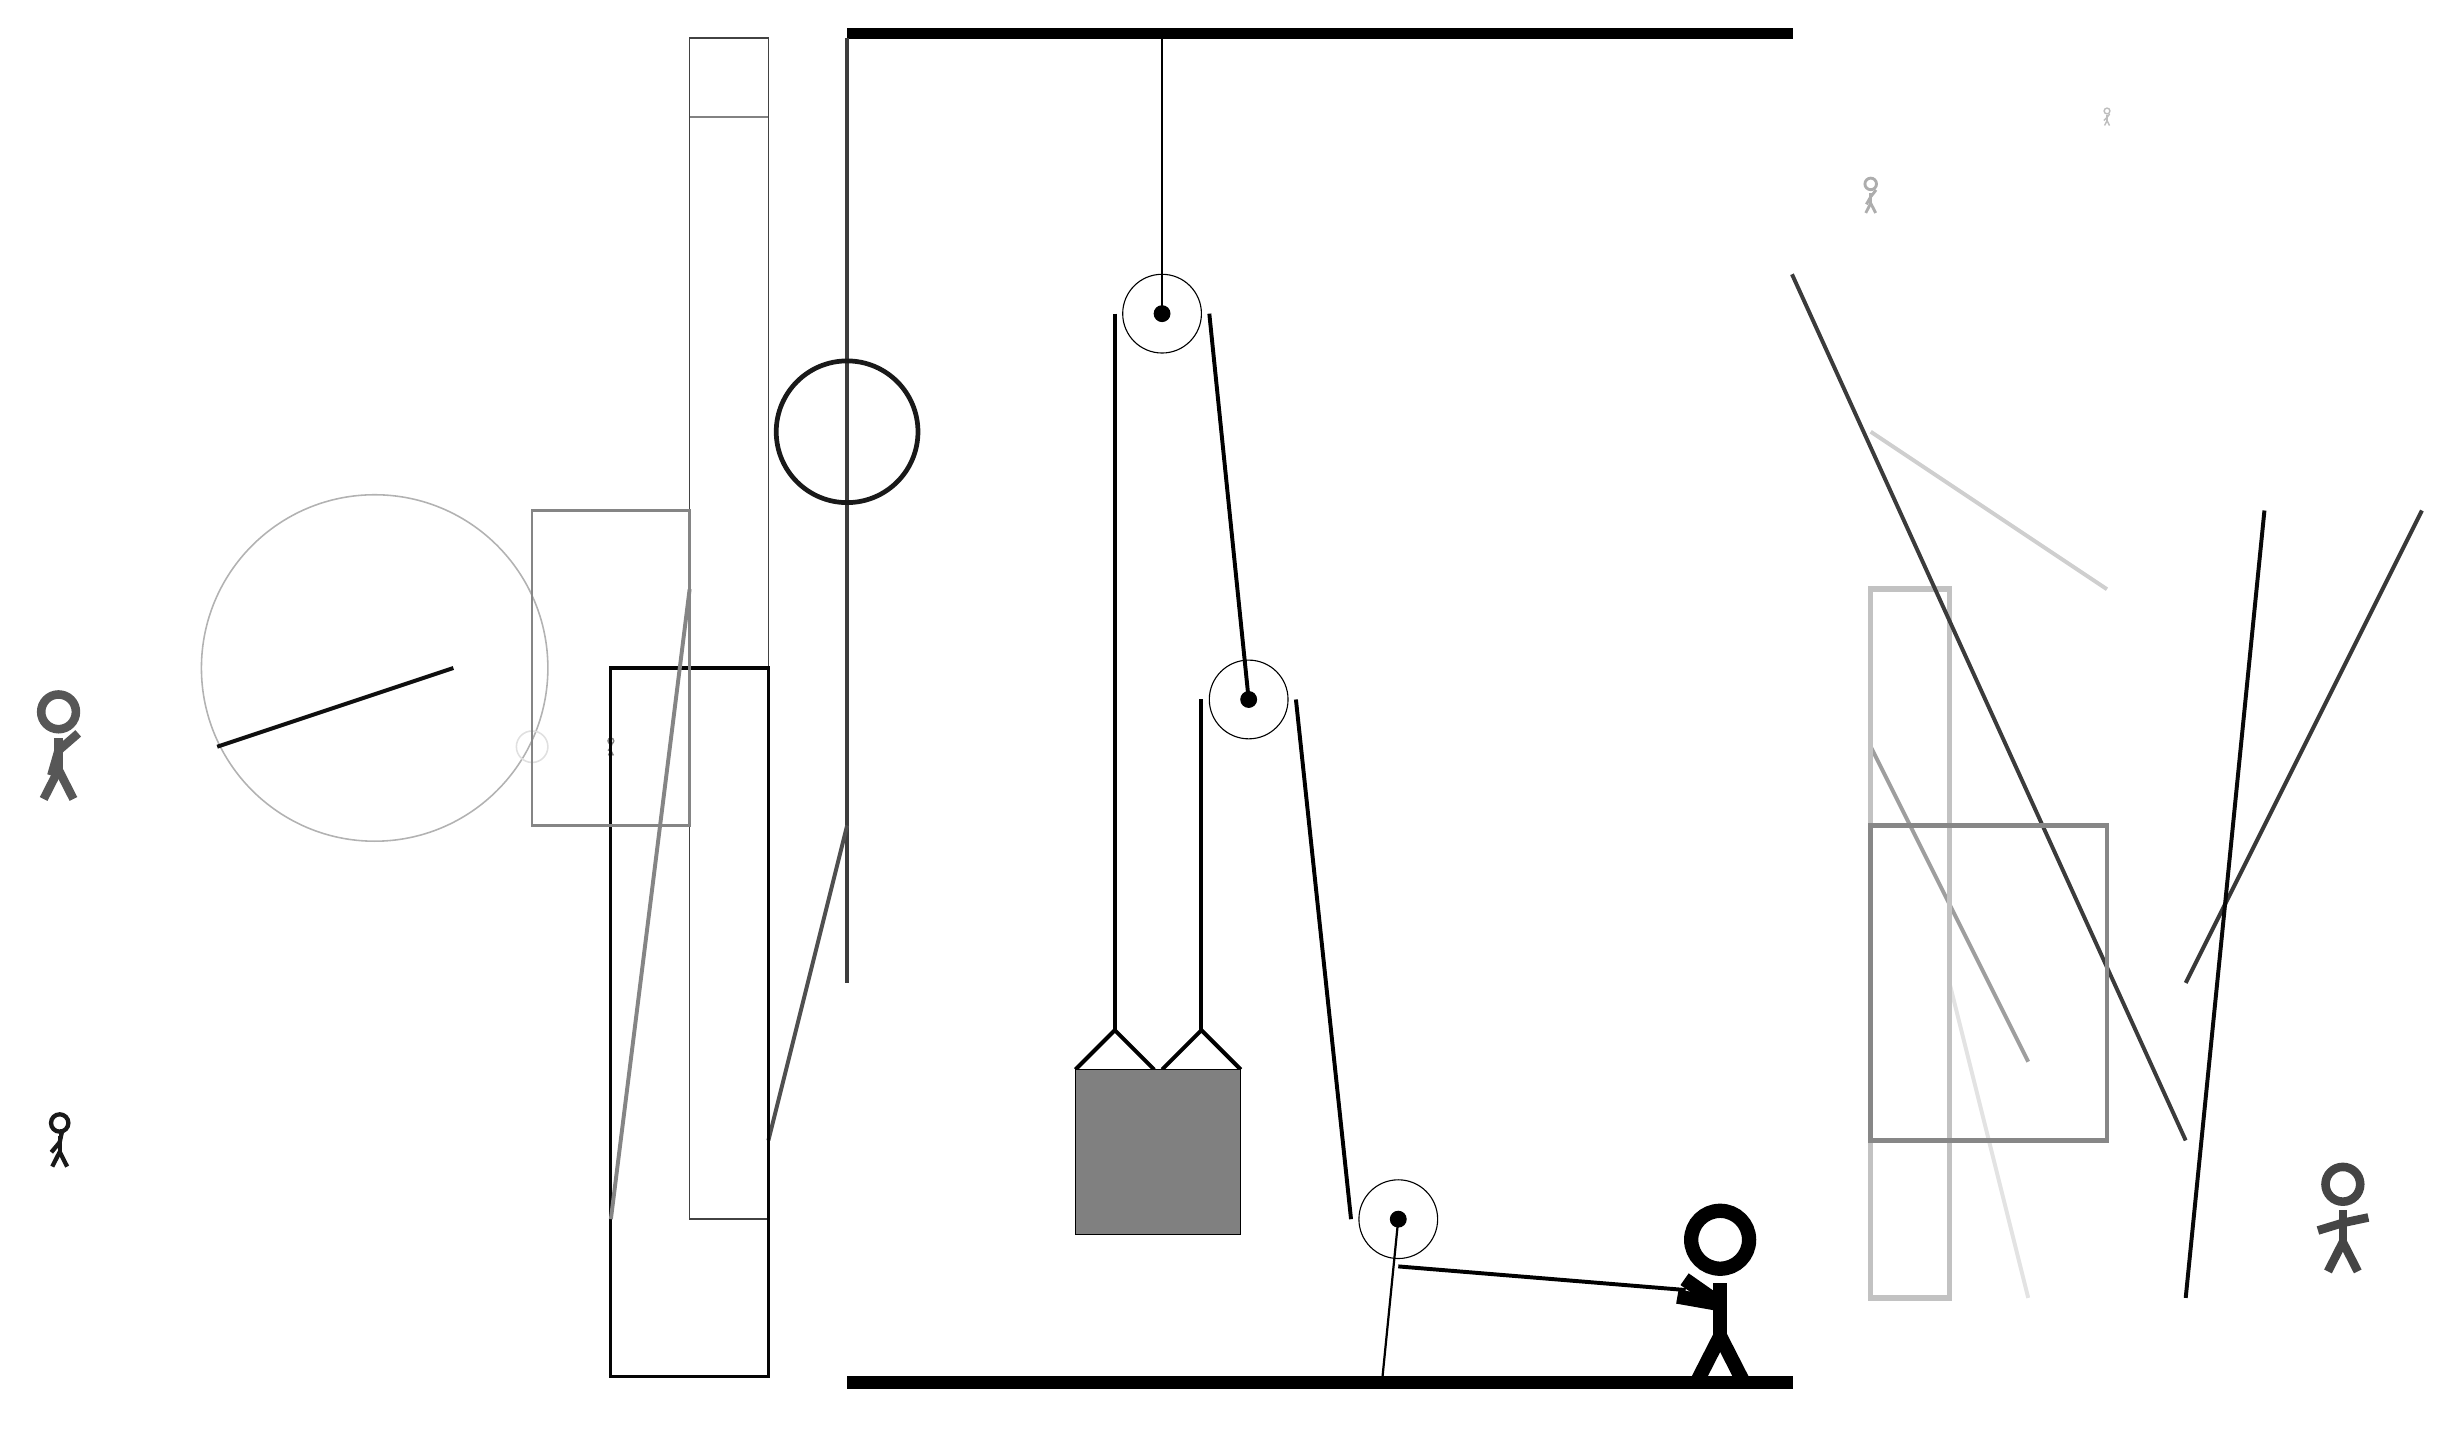
\begin{tikzpicture}
			%%%%% START %%%%%
			
			\draw[fill=black] (-2, 14) rectangle (10, 14.125);
			
			\draw (2, 10.5) circle (0.5);
			\draw[fill=black] (2, 10.5) circle (0.1);
			\draw[thick] (2, 10.5) -- (2, 14);
			
			\draw (3.1, 5.6) circle (0.5);
			\draw[fill=black] (3.1, 5.6) circle (0.1);
			
			\node[line width=0.6mm, color=black!48] at (-5, 5) {\Strichmaxerl[1][49][73]};
			
			\draw[line width=0.5mm, color=black!19](11, 9) -- (14, 7);
			\node[line width=0.5mm, color=black!26] at (14, 13) {\Strichmaxerl[1][45][53]};
			\draw [line width=0.2mm, color=black!30](-8, 6) circle (2.2);
			\draw[line width=0.5mm, color=black!76](-2, 14) -- (-2, 2);
			
			\draw[line width=0.5mm, color=black!69](-2, 4) -- (-3, 0);
			\draw[line width=0.2mm, color=black!49] (-4, 13) rectangle (-3, -1);
			\draw[line width=0.5mm, color=black!38](11, 5) -- (13, 1);
			\node[line width=0.5mm, color=black!32] at (11, 12) {\Strichmaxerl[2][60][52]};
			\draw[line width=0.5mm, color=black!94](-7, 6) -- (-10, 5);
			\draw[line width=0.2mm, color=black!74] (-3, -1) rectangle (-4, 14);
			\node[line width=0.5mm, color=black!66] at (-12, 5) {\Strichmaxerl[6][74][41]};
			\draw[line width=0.5mm, color=black!78](15, 2) -- (18, 8);
			
			\draw[line width=0.4mm, color=black!98] (-3, 6) rectangle (-5, -3);
			\node[line width=0.3mm, color=black!73] at (17, -1) {\Strichmaxerl[6][17][12]};
			\draw [line width=0.2mm, color=black!12](-6, 5) circle (0.2);
			\draw[line width=0.5mm, color=black!11](13, -2) -- (12, 2);
			\draw[line width=0.5mm, color=black!48](-4, 7) -- (-5, -1);
			\draw[line width=0.7mm, color=black!24] (12, 7) rectangle (11, -2);
			\draw[line width=0.3mm, color=black!48] (-4, 8) rectangle (-6, 4);
			\draw[line width=0.5mm, color=black!97](15, -2) -- (16, 8);
			
			\draw [line width=0.6mm, color=black!90](-2, 9) circle (0.9);
			\draw[line width=0.5mm, color=black!77](15, 0) -- (10, 11);
			\draw[line width=0.6mm, color=black!47] (11, 4) rectangle (14, 0);
			\node[line width=0.7mm, color=black!90] at (-12, 0) {\Strichmaxerl[3][50][78]};
			
			
			\draw (5, -1) circle (0.5);
			\draw[fill=black] (5, -1) circle (0.1);
			\draw[thick] (5, -1) -- (4.8, -3);
			
			\draw[line width = 0.5mm]  (0.9, 0.9) -- (1.4, 1.4) -- (1.9, 0.9);
			\draw[line width = 0.5mm]  (2.0, 0.9) -- (2.5, 1.4) -- (3.0, 0.9);
			\draw[fill=black!50] (0.9, 0.9) rectangle (3.0, -1.2);
			
			\draw[line width = 0.5mm] (1.4, 10.5) -- (1.4, 1.4);
			\centerarc[line width = 0.5mm](2, 10.5)(0:180:0.6);
			\draw[line width = 0.5mm] (2.6, 10.5) -- (3.1, 5.6);
			\draw[line width = 0.5mm] (2.5, 5.6) -- (2.5, 1.4);
			\centerarc[line width = 0.5mm](3.1, 5.6)(0:180:0.6);
			\draw[line width = 0.5mm] (3.7, 5.6) -- (4.4, -1);
			\centerarc[line width = 0.5mm](5, -1)(180:270:0.6);
			\draw[line width = 0.5mm] (5, -1.6) -- (8.65, -1.9);
			
			\node at (9, -2) {\Strichmaxerl[10][-35][170]};
			
			\draw[fill=black] (-2, -3) rectangle (10, -3.15);
			
			%%%%% END %%%%%
		\end{tikzpicture}
	\end{figure}	
\end{document}